\documentclass[12pt]{article}

\usepackage{sbc-template}
\usepackage{graphicx,url}
\graphicspath{{assets/}}
\usepackage[brazilian]{babel}
\usepackage[T1]{fontenc}
\usepackage[utf8]{inputenc}
\usepackage{amsmath,amssymb}
\usepackage{booktabs}
\usepackage{needspace}
\usepackage{minted}
\usepackage{xcolor}

\tolerance=1
\emergencystretch=\maxdimen
\hyphenpenalty=10000
\hbadness=10000
\sloppy

\definecolor{codebg}{HTML}{F6F8FA}
\definecolor{codeframe}{HTML}{D0D7DE}
\usemintedstyle{colorful}
\setminted{
  fontsize=\footnotesize,
  breaklines=true,
  breaksymbolleft={},
  autogobble=true,
  frame=single,
  framerule=0.35pt,
  rulecolor=\color{codeframe},
  bgcolor=codebg,
  baselinestretch=0.98,
  framesep=2mm
}
\renewcommand{\listingscaption}{Listagem}
\newcommand{\codetitle}[2]{%
  \refstepcounter{listing}\label{#1}%
  \noindent\textbf{\listingscaption~\thelisting: #2}\par\nopagebreak
  \vspace{0.25\baselineskip}%
}

\title{Coloração de Grafos em Rust:\\Redução do Espaço de Busca com DSATUR}

\author{Lauro Gripa Neto\inst{1}}

\address{
Centro de Ciências Tecnológicas (CCT)\\
Universidade do Estado de Santa Catarina (UDESC) -- Campus Joinville\\
Rua Paulo Malschitzki, 10 -- 89219-710 -- Joinville -- SC -- Brasil
\email{laurogripa@gmail.com}
}

\begin{document}

\maketitle

\thispagestyle{empty}
\pagestyle{empty}

\begin{resumo}
A coloração de grafos é um problema clássico de decisão NP-Completo para
$k \geq 3$, com aplicações em escalonamento, alocação de recursos e modelagem de
conflitos. Este trabalho implementa uma solução original por busca exaustiva e
uma solução otimizada exata baseada em busca de retrocesso (\textit{backtracking}), DSATUR e mapas de
bits. A
estratégia de otimização reduz a enumeração cega de $k^n$ atribuições para uma
busca podada com $T(n,k)$ estados efetivamente explorados, mantendo a precisão da
resposta. Os experimentos em Rust mostram forte redução de chamadas recursivas e
tempo de execução, embora o pior caso permaneça exponencial.
\end{resumo}
\vspace{0.5\baselineskip}
\palavraschave{Coloração de Grafos, NP-Completo, Redução de Complexidade, Rust, DSATUR.}{}

\section{Introdução}

Problemas NP-Completos representam uma fronteira importante para a análise de
algoritmos. A teoria foi estabelecida a partir do trabalho de Cook (1971) e
consolidada por Karp (1972), que apresentou reduções entre problemas
combinatórios fundamentais. Nesse
contexto, otimizar uma solução exata não significa transformar, em geral, um
problema NP-Completo em um problema polinomial. A menos que $P=NP$, o pior caso
permanece intratável. A otimização buscada neste trabalho consiste em reduzir o
espaço de busca e o custo prático de cada decisão.

O problema escolhido é a coloração de grafos. Dado um grafo simples não
direcionado $G=(V,E)$ e um inteiro $k$, deseja-se decidir se existe uma
atribuição de no máximo $k$ cores aos vértices de modo que vértices adjacentes
recebam cores diferentes. A versão de decisão é NP-Completa para $k \geq 3$,
enquanto o caso $k=2$ é resolvido em tempo polinomial por teste de bipartição.
A dificuldade computacional da coloração é documentada na literatura clássica de
problemas NP-Completos em grafos~\cite{garey1976simplified}.

O objetivo deste artigo é apresentar a solução original, sua versão otimizada,
as estratégias de redução utilizadas, os trechos de código mais relevantes e a
comparação de complexidade em notação Big O. O código completo pode ser acessado em \url{https://github.com/laurogripa/graph-coloring}.

\section{Fundamentação Teórica}

Uma coloração própria de vértices atribui uma cor a cada vértice de modo que,
para toda aresta $(u,v) \in E$, as cores de $u$ e $v$ sejam distintas. O menor
número de cores necessário para colorir um grafo é chamado número cromático.
Este trabalho considera a versão de decisão: verificar se $G$ é $k$-colorível.

O grafo de Petersen é um exemplo clássico em teoria dos grafos e serve como
ilustração compacta de uma estrutura pequena, mas não trivial~\cite{bondy2008graph}.
A Figura~\ref{fig:petersen} mostra esse grafo com uma coloração própria de três
cores, destacando visualmente a restrição central do problema: vértices
adjacentes devem receber cores distintas.

\begin{figure}[!htbp]
\centering
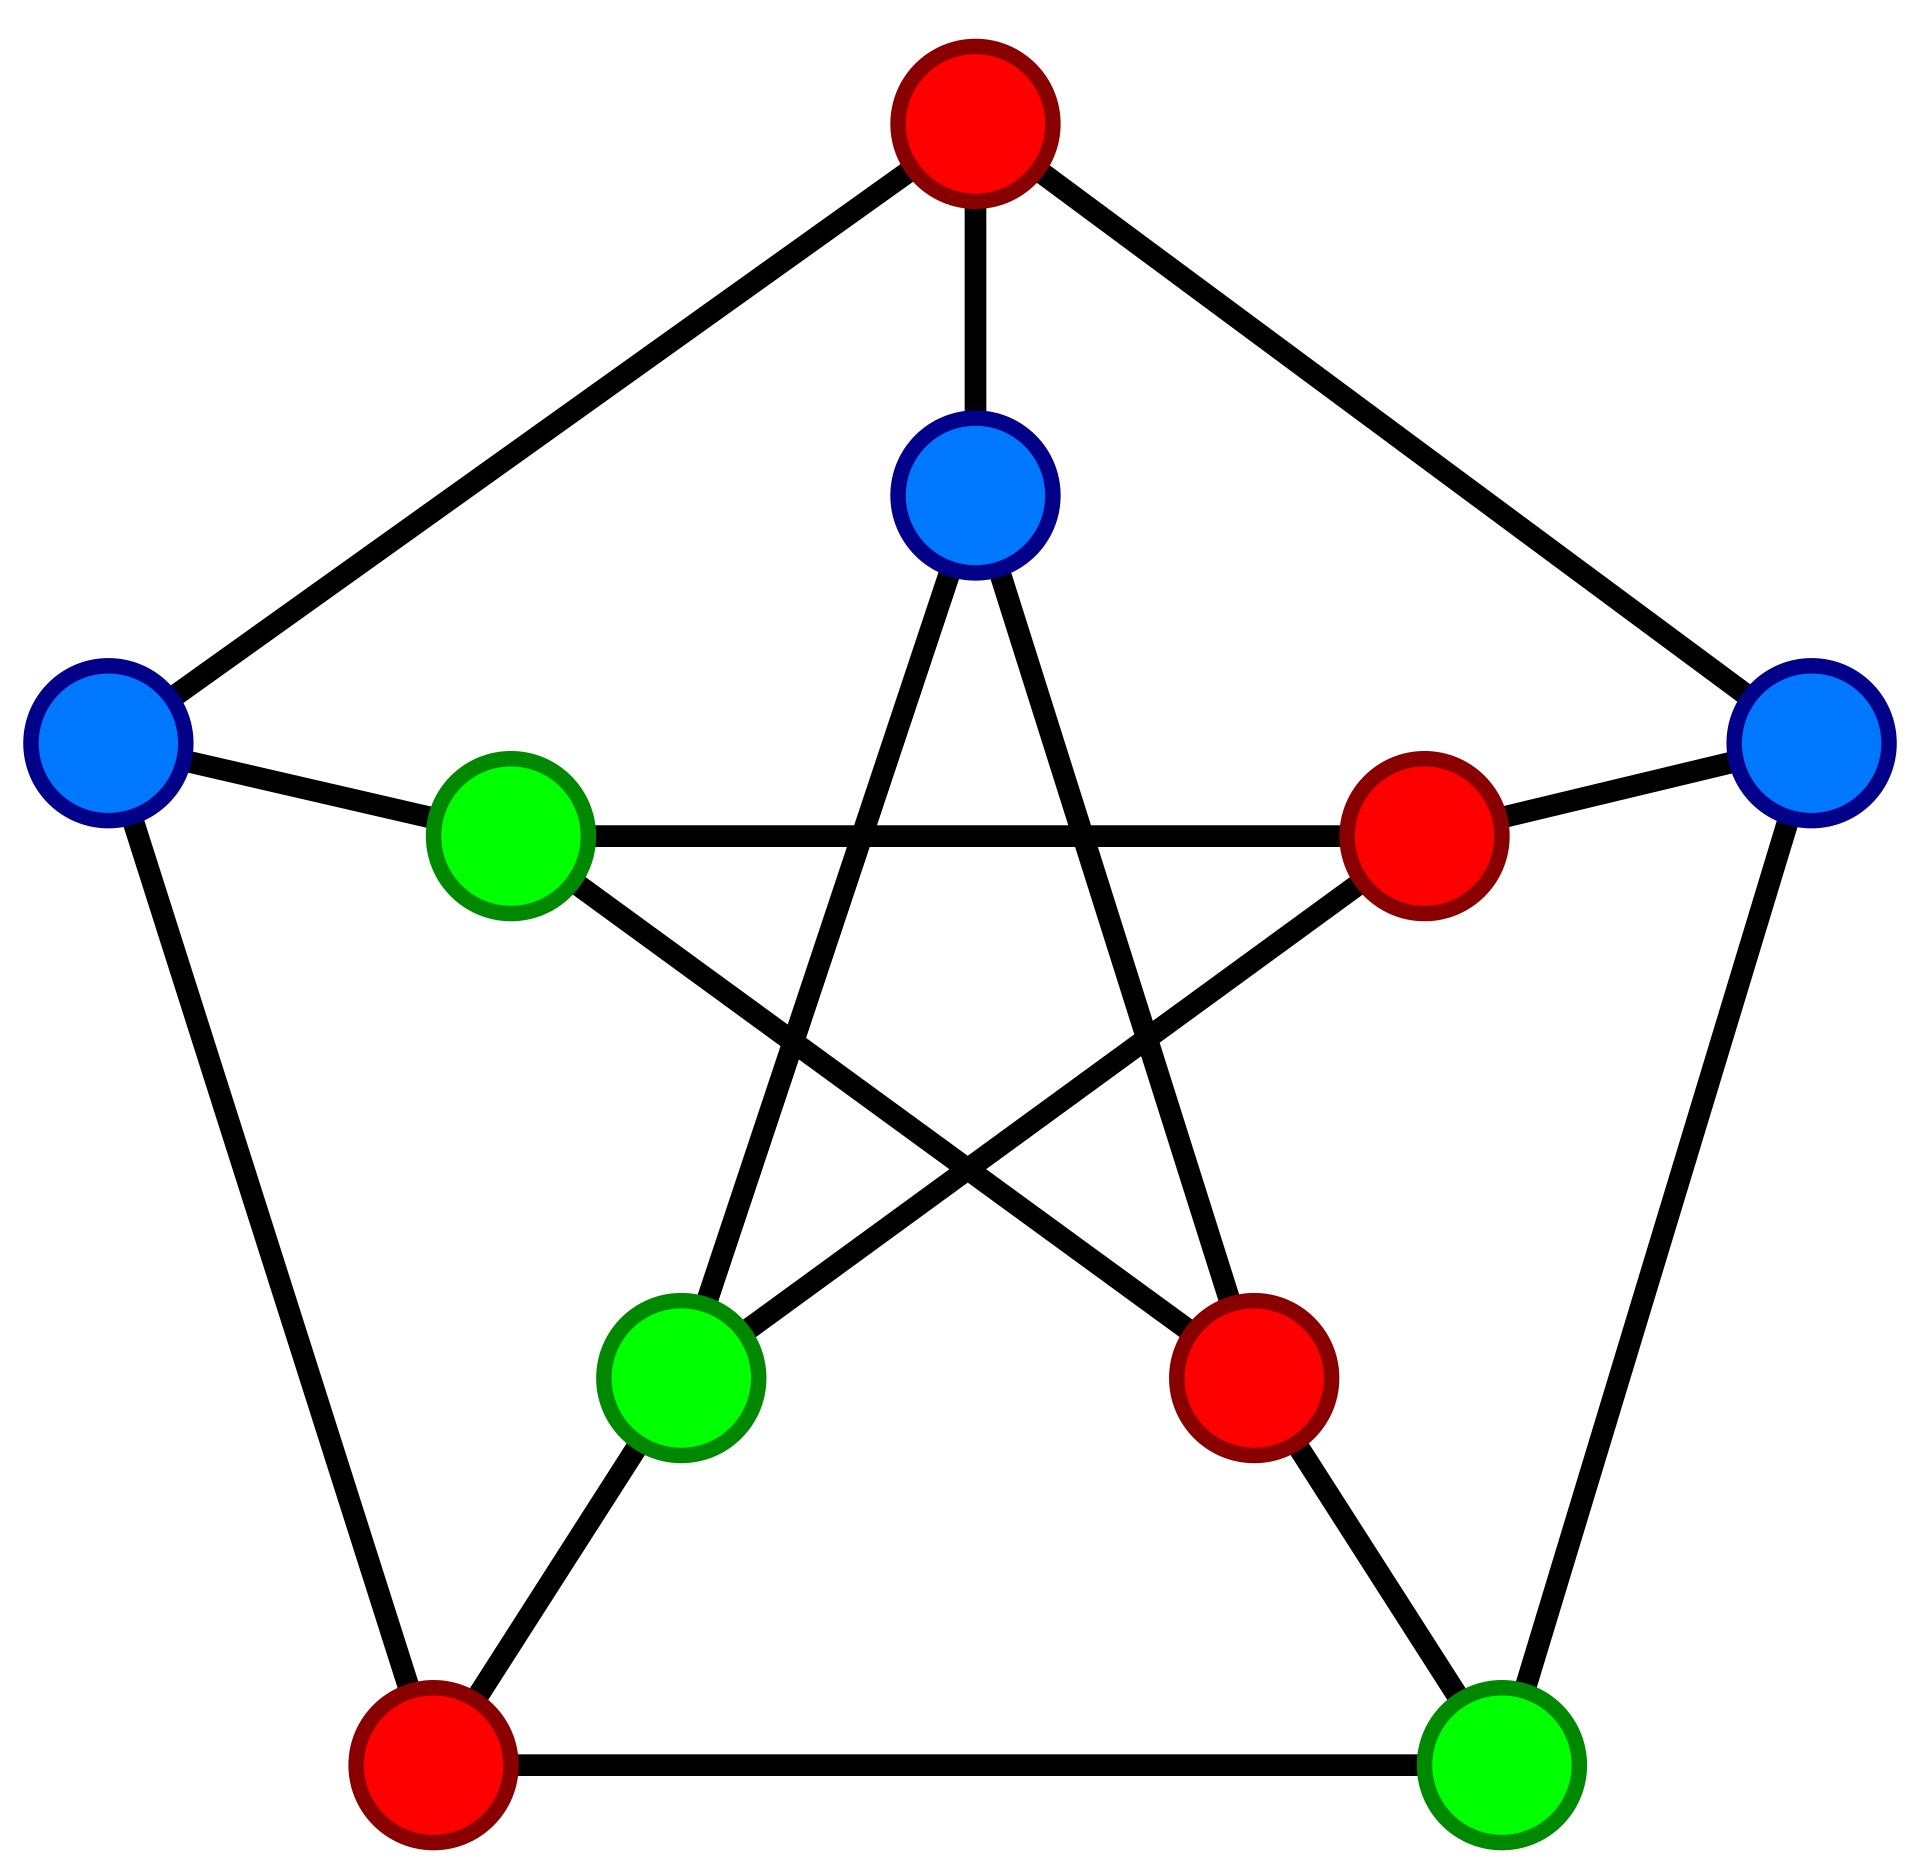
\includegraphics[width=0.38\textwidth]{Petersen_graph_3-coloring.png}
\caption{Grafo de Petersen com uma coloração própria de três cores.}
\label{fig:petersen}
\end{figure}

A análise de complexidade usa notação assintótica, seguindo a formalização
clássica de Knuth para $O$, $\Omega$ e $\Theta$~\cite{knuth1976big}. A palavra
``redução'' aparece aqui em dois sentidos distintos. Na teoria de
NP-completude, redução é uma transformação entre problemas. Na implementação
deste trabalho, redução de complexidade algorítmica significa diminuir a
quantidade de estados explorados e evitar validações completas desnecessárias.
Essa distinção é essencial: a solução otimizada reduz o custo observado e a
expressão prática da busca, mas não elimina o pior caso exponencial.

\section{Escolha da Linguagem}

A implementação foi feita em Rust porque a solução depende de representações
compactas por mapas de bits, controle explícito do estado da busca e execução
previsível. As garantias de segurança de memória formalizadas por Jung et al.
(2017) são úteis nesse contexto, pois a implementação manipula vetores, máscaras
inteiras e restaurações locais sem abrir mão de verificações estáticas. Isso
reduz o risco de erros comuns em algoritmos recursivos com muitas alterações de
estado.

Rust não altera a complexidade assintótica dos algoritmos, mas contribui para
reduzir fatores constantes. A ausência de coletor de lixo e o modelo de posse da
linguagem favorecem uma implementação em que alocações e cópias desnecessárias
são evitadas durante a busca. Em problemas exponenciais, pequenas economias por
nó visitado se acumulam ao longo de milhares ou milhões de chamadas recursivas,
o que torna relevante o foco em tempo e memória discutido empiricamente por
Pereira et al. (2017).

\section{Solução Original: Busca Exaustiva}

A solução original enumera todas as atribuições possíveis de $k$ cores para os
$n$ vértices. Cada atribuição completa é validada percorrendo as arestas do
grafo. O trecho central da implementação é mostrado na
Listagem~\ref{lst:bruteforce}.

\codetitle{lst:bruteforce}{Núcleo da busca exaustiva.}
\begin{minted}{rust}
fn brute_force_rec(graph: &Graph, k: usize, index: usize,
                   colors: &mut [usize], metrics: &mut SearchMetrics)
                   -> Option<Vec<usize>> {
    metrics.recursive_calls += 1;

    if index == colors.len() {
        metrics.complete_assignments += 1;
        if validate_coloring(graph, colors) {
            return Some(colors.to_vec());
        }
        return None;
    }

    for color in 0..k {
        colors[index] = color;
        if let Some(solution) =
            brute_force_rec(graph, k, index + 1, colors, metrics) {
            return Some(solution);
        }
    }
    None
}
\end{minted}

Como existem $k^n$ atribuições completas e cada validação percorre vértices e
arestas, a complexidade da solução original é:

\[
O(k^n \cdot (n + m)).
\]

Essa abordagem é exata, mas avalia muitas atribuições que poderiam ser
descartadas antes de serem completadas.

\section{Solução Otimizada: Backtracking com DSATUR}

A versão otimizada também é exata, mas reduz o espaço de busca. A primeira
estratégia é a busca de retrocesso (\textit{backtracking}) incremental: assim
que uma cor entra em conflito com um vizinho já colorido, o ramo é descartado. A
segunda estratégia é a escolha do próximo vértice por grau de saturação, ideia
central do DSATUR. Brélaz (1979)
propôs o método, e Lewis (2021) discute aplicações modernas de coloração. O
vértice escolhido é aquele que já possui mais
cores distintas em sua vizinhança; em caso de empate, usa-se o maior grau.

A implementação mantém, para cada vértice, uma máscara de cores proibidas. Isso
evita recalcular a saturação percorrendo toda a vizinhança a cada tentativa. A
Listagem~\ref{lst:dsatur} mostra o núcleo da busca otimizada.

\clearpage
\codetitle{lst:dsatur}{Núcleo da busca otimizada com DSATUR.}
\begin{minted}{rust}
let vertex = select_dsatur_vertex_with_masks(graph, colors, forbidden_masks)?;
let available = available_colors_mask(forbidden_masks[vertex], k);
if available == 0 {
    return None;
}

for color in 0..k {
    if available & (1_u64 << color) == 0 {
        continue;
    }

    colors[vertex] = color;
    let changed_masks =
        apply_color_to_neighbors(graph, colors, forbidden_masks, vertex, color);

    if let Some(solution) =
        dsatur_rec(graph, k, colors, forbidden_masks, colored_count + 1, metrics) {
        return Some(solution);
    }

    rollback_forbidden_masks(forbidden_masks, changed_masks);
    colors[vertex] = usize::MAX;
}
\end{minted}

A escolha do vértice e a atualização incremental das máscaras aparecem na
Listagem~\ref{lst:masks}.

\codetitle{lst:masks}{Seleção por saturação e atualização de mapas de bits.}
\begin{minted}{rust}
fn select_dsatur_vertex_with_masks(graph: &Graph, colors: &[usize],
                                   forbidden_masks: &[u64]) -> Option<usize> {
    (0..graph.vertex_count())
        .filter(|&v| colors[v] == usize::MAX)
        .max_by_key(|&v| {
            (forbidden_masks[v].count_ones() as usize,
             graph.degree(v), std::cmp::Reverse(v))
        })
}

fn available_colors_mask(forbidden_mask: u64, k: usize) -> u64 {
    let all_colors = if k == 64 { u64::MAX } else { (1_u64 << k) - 1 };
    all_colors & !forbidden_mask
}
\end{minted}

Seja $T(n,k)$ o número de estados recursivos efetivamente explorados após as
podas. No pior caso, $T(n,k)$ ainda pode ser $O(k^n)$. Entretanto, nas
instâncias em que as restrições aparecem cedo, $T(n,k)$ fica muito abaixo de
$k^n$. Como a implementação usa mapas de bits de 64 bits, operações de máscara
são tratadas como constantes; a escolha do vértice custa $O(n)$ e a atualização dos
vizinhos custa $O(\Delta)$, onde $\Delta$ é o grau máximo. Assim, a complexidade
da versão otimizada pode ser expressa como:

\[
O(T(n,k) \cdot (n + k + \Delta)).
\]

Como $\Delta \leq n$, uma forma simplificada é
$O(T(n,k) \cdot (n+k))$. A redução ocorre porque a busca deixa de validar
$k^n$ atribuições completas e passa a explorar apenas os ramos que sobrevivem às
podas. O pior caso continua exponencial, mas a complexidade observada passa a
depender de $T(n,k)$, não da enumeração cega completa.

\section{Referência Heurística}

Proposto por Welsh e Powell (1967), o algoritmo Welsh-Powell foi utilizado como
referência heurística. Ele ordena vértices por grau decrescente e colore
conjuntos de vértices não adjacentes com a mesma cor. Sua complexidade típica é
$O(n^2 + m)$, mas ele não decide $k$-coloração com garantia: pode usar mais
cores do que o necessário. Por isso, Welsh-Powell aparece apenas como referência
de velocidade, não como solução otimizada principal.

\section{Experimentos e Resultados}

Os experimentos foram executados com:

\begin{minted}{bash}
cargo test
cargo run --release --bin benchmark
\end{minted}

Cada caso foi medido 25 vezes em modo otimizado; a tabela mostra o tempo
médio. As chamadas recursivas e atribuições completas são determinísticas para a
mesma instância. A busca exaustiva foi limitada a grafos de até 12 vértices.

\begin{table}[H]
\centering
\caption{Comparação experimental entre busca exaustiva e DSATUR}
\label{tab:resultados}
\footnotesize
\begin{tabular}{llrrrrr}
\toprule
Algoritmo & Caso & Arestas & Colorível & Chamadas & Atrib. & Tempo (ms) \\
\midrule
DSATUR & $n=8$, $k=3$, $d=0{,}30$ & 7 & Sim & 9 & 1 & 0,000525 \\
Exaustivo & $n=8$, $k=3$, $d=0{,}30$ & 7 & Sim & 404 & 266 & 0,001375 \\
\midrule
DSATUR & $n=10$, $k=3$, $d=0{,}35$ & 17 & Não & 16 & 0 & 0,001747 \\
Exaustivo & $n=10$, $k=3$, $d=0{,}35$ & 17 & Não & 88573 & 59049 & 0,362355 \\
\midrule
DSATUR & $n=12$, $k=3$, $d=0{,}40$ & 31 & Não & 16 & 0 & 0,002560 \\
Exaustivo & $n=12$, $k=3$, $d=0{,}40$ & 31 & Não & 797161 & 531441 & 2,980557 \\
\midrule
DSATUR & $n=18$, $k=4$, $d=0{,}30$ & 57 & Não & 257 & 0 & 0,040082 \\
DSATUR & $n=24$, $k=4$, $d=0{,}25$ & 63 & Sim & 25 & 1 & 0,003647 \\
\bottomrule
\end{tabular}
\end{table}

No caso $n=12$, $k=3$, a busca exaustiva realizou 797161 chamadas recursivas e
avaliou 531441 atribuições completas. A versão otimizada encerrou a decisão após
16 chamadas. Essa diferença ilustra a redução de complexidade prática: a poda
impede que a maioria das combinações seja sequer completada.

\section{Análise Crítica}

A efetividade da otimização aparece em duas frentes. Primeiro, a seleção por
saturação tende a escolher cedo os vértices mais restritos, aumentando a chance
de detectar conflitos no início da busca. Segundo, os mapas de bits reduzem o
custo de consultar cores proibidas, substituindo verificações repetidas de vizinhança por
operações de máscara.

A principal limitação é teórica: por se tratar de um problema NP-Completo para
$k \geq 3$, a versão exata ainda possui pior caso exponencial. Existem instâncias
em que as podas não eliminam grande parte da árvore de busca. Além disso, a
representação por \texttt{u64} limita diretamente a implementação a 64 vértices e 64
cores; grafos maiores exigiriam vetores de palavras ou uma biblioteca de
mapas de bits.

Quanto ao compromisso entre tempo de execução e precisão, a versão DSATUR mantém
precisão total: ela decide corretamente se existe uma $k$-coloração. O custo é
manter uma busca potencialmente exponencial. Welsh-Powell, por outro lado, é
muito rápido, mas perde garantia de precisão para o problema de decisão. Assim,
a solução otimizada é recomendada quando a resposta exata é necessária em grafos
pequenos ou médios; heurísticas são mais adequadas quando uma coloração boa,
mas não necessariamente ótima ou decisória, é suficiente.

\section{Conclusão}

O trabalho implementou uma solução original e uma solução otimizada para
$k$-coloração de grafos. A busca exaustiva possui complexidade
$O(k^n \cdot (n+m))$, pois completa e valida atribuições de cores. A versão
otimizada usa busca de retrocesso, DSATUR e mapas de bits para reduzir o espaço
explorado a $T(n,k)$ estados, com complexidade $O(T(n,k)\cdot(n+k+\Delta))$.
Essa estratégia não muda o pior caso exponencial, mas reduz fortemente a
complexidade prática nas instâncias testadas, preservando a exatidão da resposta.

\bibliographystyle{sbc}
\nocite{brelaz1979new,lewis2021guide,welsh1967upper,jung2017rustbelt,pereira2017energy}
\bibliography{ref}

\end{document}
